\documentclass[11pt,a4paper]{article}

\usepackage[utf8]{inputenc}
\usepackage[T1]{fontenc}
\usepackage[margin=2.5cm]{geometry}
\usepackage{graphicx}
\usepackage{booktabs}
\usepackage{hyperref}
\usepackage[numbers,sort&compress]{natbib}
\usepackage{amsmath}
\usepackage{longtable}
\usepackage{array}
\usepackage{caption}
\usepackage{subcaption}
\usepackage{xcolor}
\usepackage{listings}
\usepackage{microtype}
\usepackage{parskip}

\lstset{
  basicstyle=\small\ttfamily,
  breaklines=true,
  breakatwhitespace=false,
  frame=single,
  backgroundcolor=\color{gray!10},
  xleftmargin=1em,
  xrightmargin=1em,
}

\hypersetup{
  colorlinks=true,
  linkcolor=blue,
  urlcolor=blue,
  citecolor=blue,
}

\title{An end-to-end computational framework for DNA-encoded chemical library analysis}
\author{Adriano Martinelli+*, Alice Lessing+, Gary Hoppeler, Andreas Gloger, Louise Plais,, Jörg Scheuermann*\\
\small Institute of Pharmaceutical Sciences, Department of Chemistry and Applied Biosciences, ETH Zurich 8083 Zurich, Switzerland\\
\small + these authors contributed equally; *corresponding authors:; Adriano Martinelli, e-mail: adriano.martinelli@pharma.ethz.ch  Jörg Scheuermann, email: joerg.scheuermann@pharma.ethz.ch}
\date{}

\begin{document}
\maketitle

\begin{abstract}
DNA-encoded chemical libraries (DELs) have emerged as a transformative technology in drug discovery, enabling the simultaneous screening of millions to billions of individually DNA-tagged small molecules and their identification after PCR amplification and high-throughput DNA sequencing. However, the computational analysis of DEL screening data is a challenge, requiring sophisticated integration of genomics, cheminformatics, and statistical analysis workflows for which currently no general, open-source software solution is available. This protocol presents DELT-Hit (DNA-Encoded Library Technology Hit Identification), a comprehensive open-source command line tool which allows computational and experimental researchers to analyze DEL data through an intuitive command-line interface. DELT-Hit offers a pipeline that converts raw FASTQ reads into machine learning-ready chemical information by five interconnected modules: (1) adaptive sequence demultiplexing using optimized algorithms with error correction and flexible barcode handling, (2) automated chemical structure reconstruction from building block libraries using reaction SMIRKS templates with support for both single and dual display DEL architectures, (3) comprehensive molecular property calculation and descriptor generation using established cheminformatics libraries, (4) statistical analysis and hit ranking with multiple normalization strategies adapted from proven RNA-seq methodologies, and (5) integrated quality control and visualization tools specifically designed for DEL data interpretation. DELT-Hit addresses a critical computational gap identified in the DEL field and provides the standardization necessary for reproducible analysis across research groups. The protocol is accompanied by comprehensive documentation and a tutorial dataset, allowing for a consistent implementation across the rapidly growing DEL community.
\end{abstract}

Key Points

\begin{itemize}
  \item Scalability and performance: DELT-Hit is designed to handle the computational demands of modern pharmaceutical DEL campaigns, efficiently processing libraries containing millions of compounds while maintaining a user-friendly interface
  \item Comprehensive DEL architecture support: The framework provides native support for both single and dual display DEL architectures, addressing the full spectrum of current library designs used in industry and academia
  \item Validated algorithms: Integrates proven bioinformatics tools (Cutadapt for sequence processing, edgeR for statistical analysis) with specialized DEL-specific optimizations, error handling, and quality control metrics
  \item Flexible and robust design: Modular architecture accommodates diverse library formats, custom reaction templates, and building block definitions
  \item Machine learning ecosystem integration: Generates standardized, analysis-ready datasets compatible with downstream machine learning workflows for advanced hit prediction, structure-activity relationship analysis, and virtual screening applications
\end{itemize}

\subsection{Technical Overview}
DELT-Hit is implemented as a Python package organized into five core modules:

\begin{itemize}
  \item init: Project initialization and configuration management with Excel template support
  \item demultiplex: Sequence processing and demultiplexing with adaptive error correction
  \item qc: Quality control plot generation and statistical summaries
  \item report: Comprehensive reporting with sequence mapping statistics
  \item library: Chemical structure reconstruction and molecular property calculation
  \item enumerate: SMILES construction from reaction steps and building blocks
  \item properties: Molecular descriptor computation and distribution visualization
  \item represent: Chemical representation generation for downstream machine learning
  \item dashboard: Interactive data exploration and real-time visualization interface
  \item analyse: Statistical analysis and hit ranking with multiple enrichment methods
\end{itemize}

\subsection{Introduction}
DNA-encoded chemical libraries (DELs) have revolutionized modern small-molecule drug discovery by enabling the synthesis and screening of chemical spaces that would be impractical to explore using traditional high-throughput screening approaches\cite{ref1,ref2,ref3,ref4,ref5,ref6,ref7,ref8,ref9}. In analogy to biological display technologies, DEL features a direct link between a library member's phenotype (i.e., the small molecule) and genotype (i.e, the encoding DNA oligonucleotide) which allows for the simultaneous and inexpensive screening of libraries of very large sizes (millions to billions) against chosen biological targets, thus greatly facilitating hit discovery\cite{ref4,ref10}.
These affinity-based selections on targets can be automatized and have been reported in a previous Nature Protocol\cite{ref11}. At the last step of the affinity-based selection process, the DNA tags of the remaining/binding compounds need to be PCR amplified and deep-sequenced by high-throughput DNA sequencing, to reveal the frequency (code counts) of each selected library member\cite{ref11,ref7}.

As outlined in comprehensive review articles on DEL technology12,7-9, DELs are now employed by essentially all large pharmaceutical companies, and also by a multitude of academic laboratories worldwide.

Various types of DEL architectures have been developed, which can be classified as single-display and dual-display libraries, depending on the pharmacophore being displayed by just one linked DNA fragment, or jointly displayed by two strands of stably or dynamically pairing oligonucleotides\cite{ref13}. While standard DELs are usually encoded by a double stranded “DNA headpiece”, other setups feature single-stranded DNA or Y-shaped encoding systems\cite{ref14}. However, regardless of the encoding system used, after selection and PCR amplification, all displays eventually lead to double-stranded amplicons which are DNA sequenced and analyzed\cite{ref11}.

Considering the large volume of data generated, the computational analysis of DEL screening data is a critical factor, requiring sophisticated integration of genomics, cheminformatics, and statistical analysis . DEL screening data presents unique opportunities for machine learning\cite{ref15,ref16,ref17,ref18,ref19,ref20,ref21,ref22,ref23,ref24,ref25,ref26,ref27,ref28} – but also challenges that require specialized approaches distinct from conventional genomics workflows: accurate demultiplexing of complex DNA barcode combinations from sequencing reads, reconstruction of chemical structures from building block combinations defined by reaction schemes, statistical analysis of enrichment patterns across multiple selection conditions, and integration with cheminformatics workflows for hit optimization and structure-activity relationship analysis.

While individual steps of a typical DEL analysis workflow can be completed by adapting tools originally developed for RNA-seq29, these tools lack the flexibility to accommodate diverse library architectures and experimental designs. Most existing approaches do not integrate well with standard bioinformatics pipelines or provide adequate quality control mechanisms for systematic troubleshooting and validation.


\subsubsection{Development of the protocol}
As a research lab that is practicing DEL technology in all aspects (i.e., design, synthesis, target-based screening), we designed DELT-Hit to address the scale and complexity of modern DEL campaigns, supporting libraries with millions of compounds while maintaining computational efficiency and user friendliness. Its modular architecture enables workflow customization while preserving reproducibility through configuration files and standardized outputs. The framework combines established bioinformatics methods with DEL-specific optimization, provides flexible configuration for diverse library designs and experimental protocols, incorporates comprehensive quality controls at each analysis stage, and remains accessible to users with varying computational backgrounds through intuitive command-line interfaces and extensive documentation.


\begin{figure}[htbp]
\centering
\includegraphics[width=\textwidth]{figures/image1.png}
\caption{DELT-Hit is organized in several modules (blue rectangles) which integrate seamlessly with the wet-lab DEL workflow (green rectangles). The synthesis of the DEL (A.) from selected building blocks is done over iterative cycles of building block addition and encoding. DELs are then interrogated in affinity-based selection experiments (B.) against relevant biological targets. Whilst non-binding library members are washed away, DNA-encoded small molecules bound to the target can be selectively eluted. The coding information of selection eluates is then amplified by PCR and sequenced through next-generation sequencing. To reveal the identities of the selected compounds, DELT-Hit uses cutadapt\cite{ref29} to demultiplex the obtained sequencing data (C.), allowing for user-specified error rates. The obtained counts matrix tabulates sequence counts for all combinations of codes and enables resolution between different selection experiments through distinct selection codes. In parallel, in silico enumeration of library compounds (D.) can be performed using SMILES to represent building block structures and customizable reaction SMIRKS to define the coupling steps. Properties and molecular descriptors for the compounds comprised within the in silico libraries can be computed (E.) to assess drug-likeness and overall library properties. Importantly, DELT-Hit can already be used to guide library planning and building block selection through its library enumeration (D.) and property calculation (E.) modules by generating prospective libraries in silico and analysing their chemical properties. Hit analysis by DELT-Hit (F.) integrates the sequencing data within the counts matrix and the molecular information generated through library enumeration and property calculation. DELT-Hit also enables an assessment of data quality, through quality control metrics giving insight into retention of reads during demultiplexing, barcode coverage and reproducibility between replicates. To evaluate hits, library members can be ranked according to their enrichment, using several ranking methods such as edgeR and counts and the dashboard provides an intuitive visualisation of selection fingerprints and enables their interactive exploration. Finally, DELT-Hit provides the obtained enrichment data and representations of library compounds as Morgan fingerprints and BERT embeddings in a format ready for downstream machine learning applications.}
\label{fig:figure1}
\end{figure}
The framework integrates multiple specialized modules (Figure 1), including sequence demultiplexing via adapted Cutadapt workflows\cite{ref29}; chemical compound representation as SMILES\cite{ref30,ref31,ref32} and chemical reaction step definitions as reaction SMIRKS\cite{ref33,ref34} implemented in RDKit\cite{ref35}; statistical analysis with edgeR\cite{ref36}; comprehensive molecular property calculations for drug-likeness assessment; and interactive visualization dashboards for real-time data exploration and hit interpretation.

This modular architecture enables users to execute complete workflows for routine analysis or utilize individual components for specialized applications. Each stage of the pipeline produces an executable script, allowing users to easily adapt the workflow to more complex experimental designs and custom settings, while maintaining reproducibility through standardized configuration files and output formats. The protocol has been successfully validated across diverse DEL architectures including multi-cycle libraries, hybridized libraries combining independent synthetic routes, and large-scale pharmaceutical screens with millions of compounds.


\subsubsection{Overview of the procedure}
The DELT-Hit protocol is organized into six sequential stages executed through a command-line interface designed to support both computational chemists experienced with bioinformatics tools and experimental scientists new to DEL data analysis:

(i) Project setup and library specification (Steps 1--3): Configuration file creation from Excel templates, library architecture definition, and experimental metadata specification.

(ii) Sequence demultiplexing and quality assessment (Steps 4--7): High-throughput sequence processing, barcode identification with error correction, and quality control metric generation.

(iii) Data visualization and interpretation (Step 8): Interactive dashboard exploration of raw count data to identify selections of interest.

(iv) Selection-centric enumeration and analysis (Steps 9--10): Automated SMILES generation and molecular property calculation for the top enriched compounds of a chosen selection.

(v) Statistical analysis and hit detection (Steps 12--13): Enrichment analysis using established RNA-seq methods, hit ranking with multiple statistical approaches, and result validation.

(vi) Full library enumeration and machine learning representations (Step 14): Optional full-library enumeration and generation of molecular fingerprints and embeddings for downstream machine learning workflows.


\subsubsection{Applications of the method}
The DELT-Hit framework accommodates various library architectures from simple two-cycle libraries to complex multi-branch synthetic schemes and has been successfully applied across our diverse DEL screening campaigns:

A single-display DEL of two diversity elements comprising 366,600 glutamic acid derivatives (GB-DEL) was encoded in single-stranded DNA format and was tested in affinity-based selections, eventually allowing for the de novo identification of specific binders against several pharmaceutically relevant proteins. In addition, the GB-DEL was used for affinity maturation in dual display fashion by combining it with low affinity hits displayed on a pairing strand\cite{ref37}.

A further single-display DEL of two diversity elements 670,752 derivatives based on 2-azido-3-iodophenylpropionic acid scaffold (NF-DEL) which was also encoded in single-stranded DNA format and used for investigating the impact of stereo- and regiochemistry on ligand discovery. The NF-DEL was tested for a set of protein targets of pharmaceutical relevance, yielding selective enzyme inhibitors and binders to tumor-associated antigens, which enabled conditional chimeric antigen receptor T-cell activation and tumor targeting\cite{ref38}.

A single-display, double-stranded proof-of-principle 1,100 member DEL of three amino acid diversity elements was synthesized using a novel solid phase-based approach on magnetic beads featuring a final release of the library from the support. This release was enabled by both simple cleavage of the connecting linker to the solid support, resulting in a standard DEL (unpurified DEL), as well as by installing a terminal second linker to the bead, followed by cleavage of the first linker (thereby releasing incomplete synthetic structures) and then the second linker, releasing only the desired structures (self-purified DEL). Both versions of the DEL were then tested in affinity-based selections against carbonic anhydrase II and IX, revealing a markedly improved enrichment of the positive control for the self-purified DEL version. While the final synthetic yields of the individual library members of the self-purified DEL still vary depending on the individual building block, unlike standard DELs, the yields of chemical display of the self-purified DEL can be assessed by DNA sequencing of the unselected library because synthesis and encoding yields correlate. Furthermore, as synthesis occurs on solid support, this PureDEL technology allows the use of anhydrous reaction conditions, thereby enabling higher conversion yields and the implementation of – so far DEL-incompatible – water-free chemistry\cite{ref39}.

A dual display, DEL encoded Self-Assembling Chemical (ESAC) Libraries of 56 million members allowed for the two displayed peptides to be connected in an incremental fashion. The DP-DEL was synthesized and tested for modulating macrocycle flexibility using a two-step cyclization strategy. By performing affinity-based selections on three different targets, specific preferences for the various degrees of flexibility were observed, i.e., a 314 nM thrombin inhibitor from the conformationally restrained macrocyclic subset of the ESAC library,  a more flexible streptavidin binder from the semi-closed conformation, as well as  binders to human alkaline phosphatase (PLAP) from the open, conventional dual-display setup. The results obtained from this approach demonstrated the utility of dual-display DEL technology for facilitating the de novo discovery of peptide ligands through flexibility-tuning\cite{ref40}.


\subsubsection{Limitations}
While DELT-Hit addresses many challenges in DEL analysis, several limitations should be considered:

\begin{itemize}
  \item Computational complexity: library size grows combinatorially with the number of diversity elements, which primarily impacts enumeration, property computation and representation. In contrast, demultiplexing complexity is limited by the number of sequencing reads, making this step largely independent of the library size.
  \item Library complexity: DELT-Hit supports arbitrary sequences of chemical reactions, provided that each synthetic route yields a single, well-defined final product, as is expected for high-quality DNA-encoded libraries. Libraries with complex architectures, such as non-standard reaction schemes, atypical building block representations, or unconventional precursor handling may require additional custom configuration and validation. In particular, the library enumeration step assumes accurate specification of reaction chemistry using reaction SMIRKS. While DELT-Hit provides templates for commonly used DEL reactions, defining library-specific SMARTS/SMIRKS may require advanced cheminformatics expertise to ensure correct product generation and structure reconstruction.
\end{itemize}

\subsection{Comparison with other methods}
Pharmaceutical companies that actively conduct DEL campaigns typically rely on internally developed or licensed software platforms that integrate sequencing, barcode decoding, hit identification, and downstream hit prioritization within proprietary ecosystems. While these systems support scalability, automation, and tight integration with experimental follow-up, they are closed-source, which restricts methodological transparency, limits user-driven customization, and hinders iterative improvement by the broader research community.

In parallel, contract research organizations (CROs) provide DEL screening as a service against user-supplied targets. These services generally return processed results without disclosing the underlying computational workflows or intermediate data products. Consequently, users have limited ability to adapt analytical procedures, interrogate intermediate outputs, or incorporate DEL informatics into their own computational pipelines.

To our knowledge, DELi\cite{ref41} is the only existing open-source software solution, including barcode decoding, enrichment analysis, and library enumeration. DELi and DELT-Hit share key design principles, such as modular architecture, transparent configuration, and integration with established bioinformatics and cheminformatics tools (e.g., Cutadapt, RDKit). However, our framework differentiates itself through several distinct capabilities:

Support for arbitrary reaction graphs for enumeration, enabling faithful reconstruction of complex synthetic schemes.

Integration of statistical models developed for RNA-seq analysis for hit calling that account for replicate structure and dispersion.

Support for arbitrary library designs, including single- and dual-display formats

Standardized output of SMILES representations for library members, facilitating downstream machine-learning workflows.

DELT-Hit explicitly and deliberately exposes intermediate data products and executable scripts, facilitating reproducibility, benchmarking, and integration, which allows users to inspect, adapt, and extend each analysis step. This positions DELT-Hit as a complementary alternative for academic and industrial users seeking industrial-scale performance without the constraints of proprietary software.


\subsection{Experimental design}

\subsubsection{Input requirements}
The DELT-Hit framework processes three primary input categories, each with specific formatting requirements that are described in the following sections in detail:

(1) Library definition files (.xlsx): Defines building block structures in SMILES format, reaction SMIRKS templates defining reaction steps, DNA constant sequences, and barcode-to-building block mapping tables. These are typically provided in Excel format with standardized sheet names for automated parsing.

(2) Raw sequencing data (fastq.gz): FASTQ files generated by Illumina or compatible sequencing platforms are supported in both compressed and uncompressed formats.

(3) Experimental metadata (.yaml): Selection condition specifications including target proteins, control experiments, and replicate groupings. This information defines the statistical comparisons and quality control parameters for downstream analysis.


\subsubsection{Library architecture considerations}
DELT-Hit supports diverse library architectures with flexible configuration options:

Single display libraries: Linear synthetic schemes where DNA tags are appended after each reaction cycle, suitable for most academic and industrial applications and focused screening campaigns.

Dual display libraries: Architectures where compounds are displayed on both complementary DNA strands, enabling higher diversity and more specialized DEL applications.

Multi-cycle libraries: Complex reaction schemes with arbitrary numbers of synthetic steps, branching reactions, and multiple building block incorporation sites.

The framework automatically validates library architecture consistency and provides warnings for potential issues such as incomplete reaction definitions or missing building blocks.


\subsubsection{Library chemistry and reaction definition}
Reaction cycles used during library construction are specified using standardized reaction SMIRKS notation provided via structured Excel configuration files. DELT-Hit translates these definitions into an explicit reaction graph that supports arbitrary reaction sequences, branching synthetic pathways, and multi-step transformations.

DELT-Hit accommodates libraries of varying complexity, including architectures with multiple reaction cycles, provided that each synthetic route resolves to a single, well-defined final product, consistent with best practices for high-quality DNA-encoded libraries. Libraries employing non-standard reaction schemes, unconventional building block representations, or complex precursor handling may require additional customization and validation.

The library enumeration process critically depends on accurate specification of reaction schemes through SMIRKS definition. Although DELT-Hit supplies validated templates for commonly used DEL reactions, library-specific adaptations often necessitate advanced cheminformatics expertise to ensure chemically correct product formation and reliable structure reconstruction.


\subsubsection{Quality control parameters}
DELT-Hit monitors comprehensive quality metrics throughout the analysis workflow:

Demultiplexing efficiency: Percentage of sequencing reads successfully assigned to valid barcode combinations, typically \textgreater{}70\% for high-quality datasets.

Barcode recovery rates: Coverage of each barcode to identify abnormalities in the demultiplexing.

Statistical significance assessment: Multiple testing correction and false discovery rate control using established RNA-seq analysis methodologies.

Replicate consistency: Correlation analysis across biological and technical replicates.

Chemical reaction validation: Strict requirements on reaction products.


\subsection{Materials}

\subsubsection{Equipment}
Computing hardware:

\begin{itemize}
  \item Minimum configuration: 8 GB RAM, 8 CPU cores, 50 GB available storage
  \item Recommended configuration: 32 GB RAM, 16 CPU cores, 100 GB available storage
  \item High-performance setup: 64 GB RAM, 32 CPU cores, 250 GB SSD storage
\end{itemize}
Operating systems:

\begin{itemize}
  \item Linux (Ubuntu 20.04+)
  \item macOS (12.0+)
  \item Windows 10/11 (with Windows Subsystem for Linux recommended)
\end{itemize}

\subsubsection{Software dependencies}
Core requirements:

\begin{itemize}
  \item Python 3.12 or higher with pip package manager
  \item Conda package manager (Miniconda or Anaconda)
  \item R statistical computing environment (version 4.1+)
  \item Git version control system (version 2.0+)
\end{itemize}
Python packages (automatically installed):

\begin{itemize}
  \item cutadapt (4.9+): Sequence adapter trimming and demultiplexing
  \item rdkit (2024.3+): Chemical structure processing and property calculation
  \item pandas (2.2+): Data manipulation and statistical analysis
  \item numpy (1.24+): Numerical computing and array operations
  \item matplotlib/seaborn: Data visualization and publication-quality plotting
  \item plotly: Interactive visualization and dashboard components
  \item scipy (1.10+): Statistical functions and optimization algorithms
\end{itemize}
R packages (manual installation required):

\begin{itemize}
  \item edgeR: Differential expression analysis adapted for count data
  \item limma: Linear modeling and empirical Bayes statistics
  \item tidyverse: Data manipulation and visualization tools
  \item GGally: Extension to ggplot2 for correlation matrices
  \item BiocManager: Bioconductor package management
\end{itemize}

\subsubsection{Input file preparation}
Required input files:


\begin{table}[htbp]
\centering
\caption{Input file specifications and sources}
\label{tab:table1}
\begin{tabular}{llll}
\toprule
File Type & Format & Description & Example Source \\
\midrule
Campaign definition & Excel (.xlsx) & Selection conditions, building blocks, reactions, constants & Laboratory records \\
Sequencing data & FASTQ (.fastq / .fasta) & Raw sequencing reads & Illumina sequencer \\
analysis.yaml & Yaml (.yaml) & Replicates used for hit identification with edgeR & Laboratory records \\
\bottomrule
\end{tabular}
\end{table}
Example datasets (available for download):

The provided example dataset is based on a toy library based on the architecture of a published library\cite{ref37}.


\begin{table}[htbp]
\centering
\caption{Tutorial datasets for protocol validation}
\label{tab:table2}
\begin{tabular}{lll}
\toprule
File & URL & Description \\
\midrule
campaign.fastq.gz & https://figshare.com/ndownloader/files/61487743 & Representative screening data for the single-stranded example \\
example-single-stranded.xlsx & https://figshare.com/ndownloader/files/61487731 & Complete library and experimental definitions for the full single-stranded workflow \\
analysis.yaml & https://figshare.com/ndownloader/files/61487728 &  \\
Supporting Material & https://doi.org/10.6084/m9.figshare.31198468 & Tutorial examples, re-analysis workflows, and output files generated by running the described protocol \\
\bottomrule
\end{tabular}
\end{table}


\subsubsection{Software installation}
The following installation procedure needs to be performed once before running the DELT-Hit protocol and is executed entirely from the command line. All subsequent analyses are likewise performed via terminal-based commands within the same software environment.


\paragraph{Step 1: Install Git version control system}

Git is required to download the DELT-Hit package from the GitHub repository.

For macOS:


\begin{lstlisting}
# Install using Homebrew (recommended)
brew install git

# Or download from: https://git-scm.com/download/mac
\end{lstlisting}
For Linux (Ubuntu/Debian):


\begin{lstlisting}
sudo apt-get update
sudo apt-get install git
\end{lstlisting}
For Windows:


\begin{lstlisting}
# Download and install from: https://git-scm.com/download/win
# Then use Git Bash or Windows Subsystem for Linux (WSL)
\end{lstlisting}
Verify Git installation:


\begin{lstlisting}
git --version
# Expected output: git version 2.x.x or higher
\end{lstlisting}

\paragraph{Step 2: Environment setup with Conda}

We recommend using Miniconda package manager to create an isolated environment ensuring proper dependency management. This step only needs to be performed once.


\begin{lstlisting}
# Download and install Miniconda for your operating system
# Follow instructions at: https://docs.anaconda.com/miniconda

# Create dedicated environment (only needed once)
conda create -n delt-hit python=3.12 -y

# Activate environment (required for each new terminal session)
conda activate delt-hit
conda install pygraphviz -y

# Install DELT-Hit package
pip install git+https://git@github.com/DELTechnology/delt-hit.git
\end{lstlisting}
Note: You will need to activate the delt-hit environment (conda activate delt-hit) each time you open a new terminal session before running DELT-Hit commands. We also recommend initializing the shell with conda during installation such that the conda command is available when opening a new terminal window. Should you not be able to activate conda after the installation please refer to the Troubleshooting section for help.


\paragraph{Step 3: R environment configuration}

Statistical analysis components require R with specific Bioconductor packages. This configuration only needs to be performed once.

Open R or RStudio and execute:


\begin{lstlisting}
# Install required CRAN packages
install.packages(c("tidyverse", "GGally"))

# Install BiocManager for Bioconductor packages
if (!require("BiocManager", quietly = TRUE))
    install.packages("BiocManager")

# Install Bioconductor packages
BiocManager::install(c("edgeR", "limma"))
\end{lstlisting}

\paragraph{Step 4: Installation verification}

Verify that all components are correctly installed:


\begin{lstlisting}
# Activate environment
conda activate delt-hit

# Test core functionality
delt-hit --help

# Expected output: Help message describing the delt-hit command
\end{lstlisting}

\subsection{Procedure}

\subsubsection{Phase 1: Project initialization and configuration • TIMING 30-60 min}
The configuration file defines library structure, experimental design, and analysis parameters. DELT-Hit supports initialization from standardized Excel templates for user convenience.

In this phase, we will create a YAML configuration file from an Excel spreadsheet that contains all the information about your DEL library and experimental design.


\paragraph{Step 1 \textbar{} Prepare Excel configuration file}

Create an Excel file with multiple sheets defining your experiment. Each sheet contains specific information required for the analysis. The following sections describe the required sheets and their format. For convenience, users can start from the template provided in Table 3.


\subparagraph{1.1 Create the experiment sheet}

This sheet contains basic experiment parameters including experiment name, file paths, and computational resources.


\begin{table}[htbp]
\centering
\caption{Experiment configuration parameters}
\label{tab:table3}
\begin{tabular}{ll}
\toprule
variable & value \\
\midrule
name & template \\
fastq\_path & campaign.fastq.gz \\
save\_dir & experiments \\
num\_cores & 11 \\
\bottomrule
\end{tabular}
\end{table}
CRITICAL STEP: Use absolute paths or paths relative to your working directory for fastq\_path and save\_dir and ensure there are no trailing whitespaces.


\subparagraph{1.2 Create the selections sheet}

This sheet defines the experimental design including selection conditions, multiplexing barcodes, and replicate grouping. Each row describes an experimental setting (for example a different protein target or experimental condition like controls) and is identified by a unique combination of S0 and S1 primers to demultiplex the sequencing data into the individual experiments.


\input{tables/table4}
Required columns for demultiplexing:

\begin{itemize}
  \item name: Unique identifier for each selection
  \item S0, S1: Multiplexing barcodes for selection identification
\end{itemize}
Required columns for statistical analysis:

\begin{itemize}
  \item group: Statistical grouping (e.g., "protein", "no\_protein", "naive")
\end{itemize}
Optional columns:

\begin{itemize}
  \item operator: Person who performed the selection
  \item date: Date of selection experiment
  \item other columns can be added up to the users discretion
\end{itemize}

\subparagraph{1.3 Create the structure sheet}

This sheet defines the DNA construct architecture and error tolerance for demultiplexing.

There are three types of DNA regions:

\begin{itemize}
  \item selection: This region is used for the selection primer as defined in the selection sheet and need to be named S0 and S1.
  \item constant: These regions are used as constant regions across all DNA constructs and need to be named sequentially C0, C1, etc.
  \item building\_block: This region identifies a chemical building block used and needs to be named sequentially B0, B1, etc.
\end{itemize}
Each region in the DNA construct is identified by a unique name and a max\_error\_rate and whether indels are allowed during multiplexing can be configured for each region.


\input{tables/table5}
Column descriptions:

\begin{itemize}
  \item name: Unique identifier for each DNA region
  \item type: Region type (selection, constant, or building\_block)
  \item max\_error\_rate: Maximum allowed error rate for adapter trimming (0 = perfect match, 1.1 = \textasciitilde\{\}10\% errors)
  \item indels: Whether to allow insertions/deletions (TRUE/FALSE)
\end{itemize}
CRITICAL STEP: Selection barcodes should require perfect matches (max\_error\_rate = 0, indels = FALSE) to ensure accurate multiplexing, while constant regions can tolerate higher error rates depending on their length.


\subparagraph{1.4 Create the constant sheet}

This sheet contains the DNA sequences for all constant regions defined in the structure sheet.


\input{tables/table6}
Note: The name column must match the constant region names defined in the structure sheet.


\paragraph{Step 2 \textbar{} Define chemical building blocks and reactions}

DELT-Hit supports libraries with an arbitrary number of building blocks. For each building block region defined in the structure sheet, the user must define the used DNA codons in a sheet named according to the structure sheet (i.e. B0, B1, ..., BN). To enable library enumeration and property calculation, users must define the chemical structure of the building blocks and reactions used in the library synthesis as well.


\subparagraph{2.1 Create building block sheets (B0, B1, etc.)}

For each building block position defined in your structure sheet, create a separate sheet containing all building blocks for that position.


\input{tables/table7}
Required columns for demultiplexing:

\begin{itemize}
  \item codon: DNA barcode sequence identifying this building block
\end{itemize}
Required columns for library enumeration:

\begin{itemize}
  \item smiles: Chemical structure in SMILES notation
  \item reaction: Name of the reaction using this building block
  \item educt: Name of the compound this building block reacts with if any
  \item product: Name of the product formed
\end{itemize}

\subparagraph{2.2 Create the reactions sheet}

Only required for library enumeration. Define all chemical reactions used during library synthesis using SMARTS/SMIRKS notation\cite{ref34}. SMARTS/SMIRKS must be adapted to the building blocks used to yield a single product for each transformation. If a reaction is used several times throughout library synthesis, these must be defined as individual reactions. Table 9 demonstrates this with two amide-bond forming reactions (ABF1 and ABF2)


\begin{table}[htbp]
\centering
\caption{Reaction SMIRKS templates}
\label{tab:table8}
\begin{tabular}{ll}
\toprule
name & smirks \\
\midrule
ABF1 & [CX3:1](=[O:2])[OX2;H1].[N;\$([N;H1,H2]),\$([N;H3]);!\$([N;H1,H2][S]);!\$([NX3][CX3](=[OX1])[\#6]);!\$([NX3][CX3](=[OX1])[OX2]):4]\textgreater{}\textgreater{}[CX3:1](=[O:2])[N:4] \\
ABF2 & [CX3:1](=[O:2])[OX2;H1].[N;\$([N;H1,H2]),\$([N;H3]);!\$([N;H1,H2][S]);!\$([NX3][CX3](=[OX1])[\#6]);!\$([NX3][CX3](=[OX1])[OX2]):4]\textgreater{}\textgreater{}[CX3:1](=[O:2])[N:4] \\
SR & [\#6:1][\$([NX2-][NX2+]\#[NX1]),\$([NX2]=[NX2+]=[NX1-])]\textgreater{}\textgreater{}[\#6:1][N;H2] \\
CuAAC & [CX2:1]\#[CX2;H1:2].[N:3]=[N+:4]=[N-:5]\textgreater{}\textgreater{}[C:1]1=[C:2][N-0:3][N-0:4]=[N-0:5]1 \\
\bottomrule
\end{tabular}
\end{table}
Note: The name column must match the reaction names used in the building block sheets.


\subparagraph{2.3 Create the compounds sheet}

Only required for library enumeration. Define any additional chemical compounds (scaffolds, reagents) used in the reactions.


\input{tables/table9}

\paragraph{2.4 Create the additional reaction steps}

Only required for advanced library enumeration. If the synthesis of the library requires additional reaction steps, for example for conversion of precursor molecules or deprotection steps before reactions, those can be described in the sheet reaction\_graph. A reaction is defined by at most two educts that react through a reaction to a new product. For each additional reaction step you want to add, include a new row with the corresponding compound names and reaction names from the reactions and compounds sheet.


\input{tables/table10}
It might be necessary to define multiple reaction paths for precursors even though they share the same reaction node in theory. Table 11 demonstrates this with two scaffolds that are activated with a Staudinger reduction (SR) reaction before reacting with the building block. The definition in Table 12 adds two independent reaction paths to the reaction graph and the reaction pathway can be resolved. In contrast, using the same reaction name SR for both would result in an invalid reaction graph that defines:

scaffold\_1 + scaffold\_2 -\textgreater{} SR -\textgreater{} scaffold\_1A + scaffold\_1B


\input{tables/table11}

\paragraph{Step 3 \textbar{} Generate configuration file}

Once your Excel file is complete with all required sheets, generate the YAML configuration file:


\begin{lstlisting}
# Activate the delt-hit environment
conda activate delt-hit

# Generate configuration from Excel template
delt-hit init --excel_path=/path/to/your/experiment.xlsx
\end{lstlisting}
This command creates a YAML configuration file at save\_dir/name/config.yaml as specified in your Excel file in sheet experiment.

Expected output:


\begin{lstlisting}
Configuration created at /path/to/results/experiments/experiment-1/config.yaml
\end{lstlisting}
CRITICAL STEP: Review the generated YAML file to verify all information was parsed correctly. The YAML file will be used for all subsequent analysis steps.

TROUBLESHOOTING: While the tool supports some basic input validation it is helpful to check the following if the command fails:

\begin{itemize}
  \item All building blocks are present in the configuration file
  \item Column names match exactly as specified in the tables above
  \item Excel file was saved with the latest changes before running the command
\end{itemize}

\subsubsection{Phase 2: Sequence processing and demultiplexing • TIMING 30 min - 4 h}
This phase processes raw sequencing reads to identify and count each library member in your selection experiments.


\paragraph{Step 4 \textbar{} Configure demultiplexing parameters}

The demultiplexing parameters defined in your Excel file control how sequence reads are processed by cutadapt. Key parameters include:

\begin{itemize}
  \item max\_error\_rate: Tolerance for sequencing errors (0 = perfect match, 1.1 = \textasciitilde\{\}10\% errors)
  \item indels: Whether to allow insertions/deletions during barcode matching
\end{itemize}
As mentioned earlier, we recommend requiring exact matches for selection barcodes (max\_error\_rate = 0, indels = FALSE) to ensure accurate multiplexing, while allowing higher error rates for constant regions depending on their length.


\paragraph{Step 5 \textbar{} Prepare and execute sequence demultiplexing}

Generate the demultiplexing scripts with its dependencies and execute the analysis:


\begin{lstlisting}
# Generate Cutadapt input files and demultiplexing script
delt-hit demultiplex prepare --config_path=/path/to/config.yaml

# Execute demultiplexing
/path/to/experiment/demultiplex/cutadapt_input_files/demultiplex.sh
\end{lstlisting}
The demultiplexing process performs:

\begin{itemize}
  \item Adapter detection and trimming: Removal of sequencing adapters
  \item Barcode extraction: Sequential identification of selection and building block barcodes
  \item Quality filtering: Rejection of reads with errors exceeding defined thresholds
\end{itemize}
The produced demultiplexing executable (.sh) uses cutadapt and to process the FASTQ file and maps the sequences to the selection and codon IDs. It generates the reads\_with\_adapters.gz file that contains all sequences that have been mapped.

Performance note: Processing speed is approximately 50,000-200,000 reads/second. For a typical dataset with 50-100 million reads, expect 30 minutes to 2 hours processing time.

Expected outputs:

\begin{itemize}
  \item demultiplex/cutadapt\_output\_files/*.cutadapt.json: Detailed processing statistics for each demultiplexing step
  \item demultiplex/cutadapt\_output\_files/reads\_with\_adapters.gz: Intermediate files with extracted barcodes
\end{itemize}

\paragraph{Step 6 \textbar{} Process demultiplexing results and generate count tables}

After demultiplexing completes, aggregate the results into count tables for each selection:


\begin{lstlisting}
# Process demultiplexing output and generate count tables
delt-hit demultiplex process --config_path=/path/to/config.yaml
\end{lstlisting}
This command:

\begin{itemize}
  \item Parses the demultiplexed reads
  \item Maps barcode combinations to library members
  \item Generates count tables for each selection
  \item Saves results in standardized format
\end{itemize}
Expected outputs:

\begin{itemize}
  \item selections/[selection\_name]/counts.txt: Tab-delimited count table with columns:
  \item code\_1, code\_2,...: Building block indices
  \item name: Selection identifier
  \item count: Number of reads for this compound in this selection
  \item NOTE: alternatively, counts can be saved as \{selection\_name\}\_counts.txt by using the flag --as\_files=True. To save the counts sorted by codon ids instead of observed counts, set the flag --sort\_by\_counts=False.
\end{itemize}

\paragraph{Step 7 \textbar{} Generate quality control reports}

Assess demultiplexing quality with comprehensive statistics and visualizations:


\begin{lstlisting}
# Generate text-based quality control report
delt-hit demultiplex report --config_path=/path/to/config.yaml

# Generate quality control visualizations
delt-hit demultiplex qc --config_path=/path/to/config.yaml
\end{lstlisting}
Expected outputs:

\begin{itemize}
  \item qc/report.txt: Comprehensive text report with processing statistics
  \item qc/*.png: Quality control plots showing barcode recovery and coverage distributions
\end{itemize}

\begin{figure}[htbp]
\centering
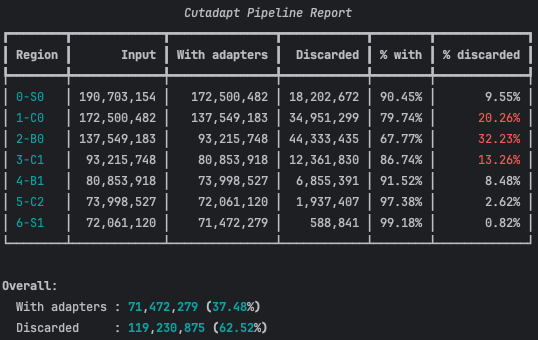
\includegraphics[width=\textwidth]{figures/image4.png}
\caption{Example report for a poor selection with only 37\% read retention. Report highlights the problematic region where more than 10\% of the reads are lost (not mapped to codons).}
\label{fig:figure4}
\end{figure}

\begin{figure}[htbp]
\centering
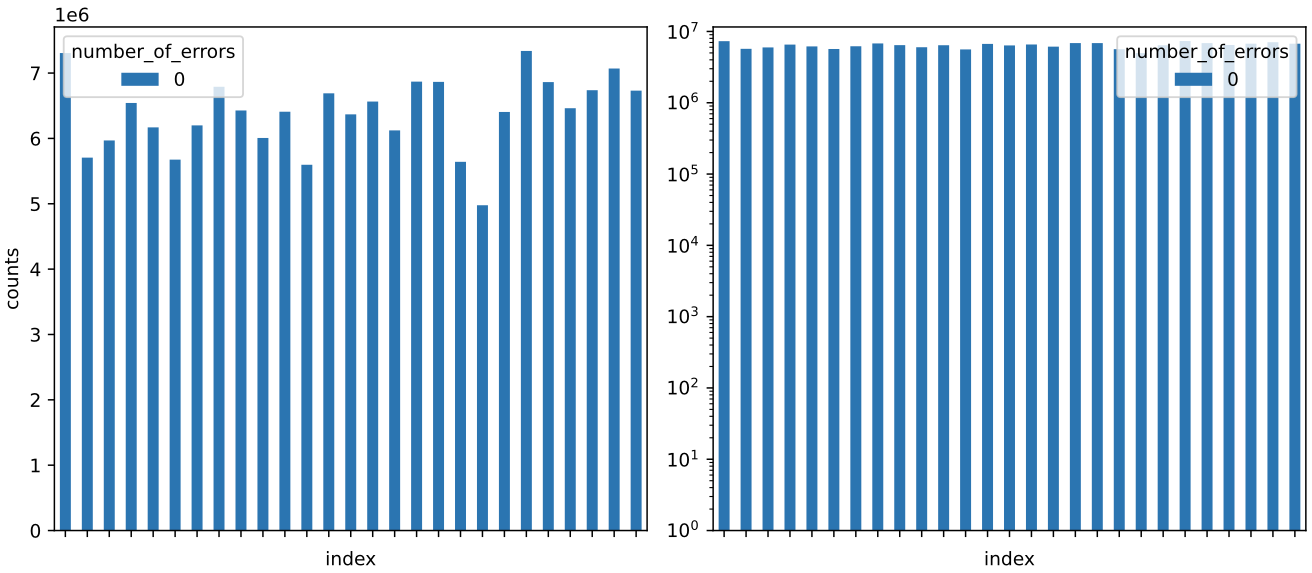
\includegraphics[width=\textwidth]{figures/image5.png}
\caption{Stacked bar plots showing the number of reads per index position for selection or barcode codons as defined in the Excel file. Absolute read counts are shown on the right, and log-transformed counts on the left. For each index position, reads are displayed as stacked segments according to the number of sequencing errors. (TOP) Stacked barplot for the assigned counts to the different selection codons of S0. (BOTTOM) Stacked barplot for read assignment to constant region C0, in orange are the number of reads that were mapped to this region with 1 error, in blue the number of reads that were mapped with 0 errors.}
\label{fig:figure5}
\end{figure}
Quality assessment criteria:

\begin{itemize}
  \item Read retention: \textgreater{}70\% of input reads should be successfully assigned
  \item Barcode coverage: Most building blocks should have \textgreater{}0 reads
\end{itemize}
TROUBLESHOOTING: Low read retention (\textless{}50\%) may indicate:

\begin{itemize}
  \item Incorrect barcode sequences in configuration
  \item Poor sequencing quality
  \item Poor library quality
\end{itemize}

\subsubsection{Phase 3: Data visualization and interpretation • TIMING 15-60 min}
The interactive dashboard provides real-time exploration of raw count data and experimental metadata.


\paragraph{Step 8 \textbar{} Launch interactive analysis dashboard}

Visualize demultiplexing results and explore count distributions:


\begin{lstlisting}
delt-hit dashboard --config_path=/path/to/config.yaml --counts_path=/path/to/experiment/selections/CA_P1/counts.txt

# Dash is running on http://127.0.0.1:8050/  # copy paste into browser
# * Serving Flask app 'delt_hit.cli.dashboard.api'
# * Debug mode: on
\end{lstlisting}
This command starts a server interface that can be opened from a web browser (typically at http://localhost:8050). Stop the server with ctrl+c or by closing the terminal.

Dashboard features:

\begin{itemize}
  \item Experimental metadata display: Selection conditions, target information, and experimental parameters
  \item Count distribution visualization: Scatter/Histograms and summary statistics for the selected condition
  \item Interactive filtering: Explore specific regions of the count distribution
\end{itemize}

\begin{figure}[htbp]
\centering
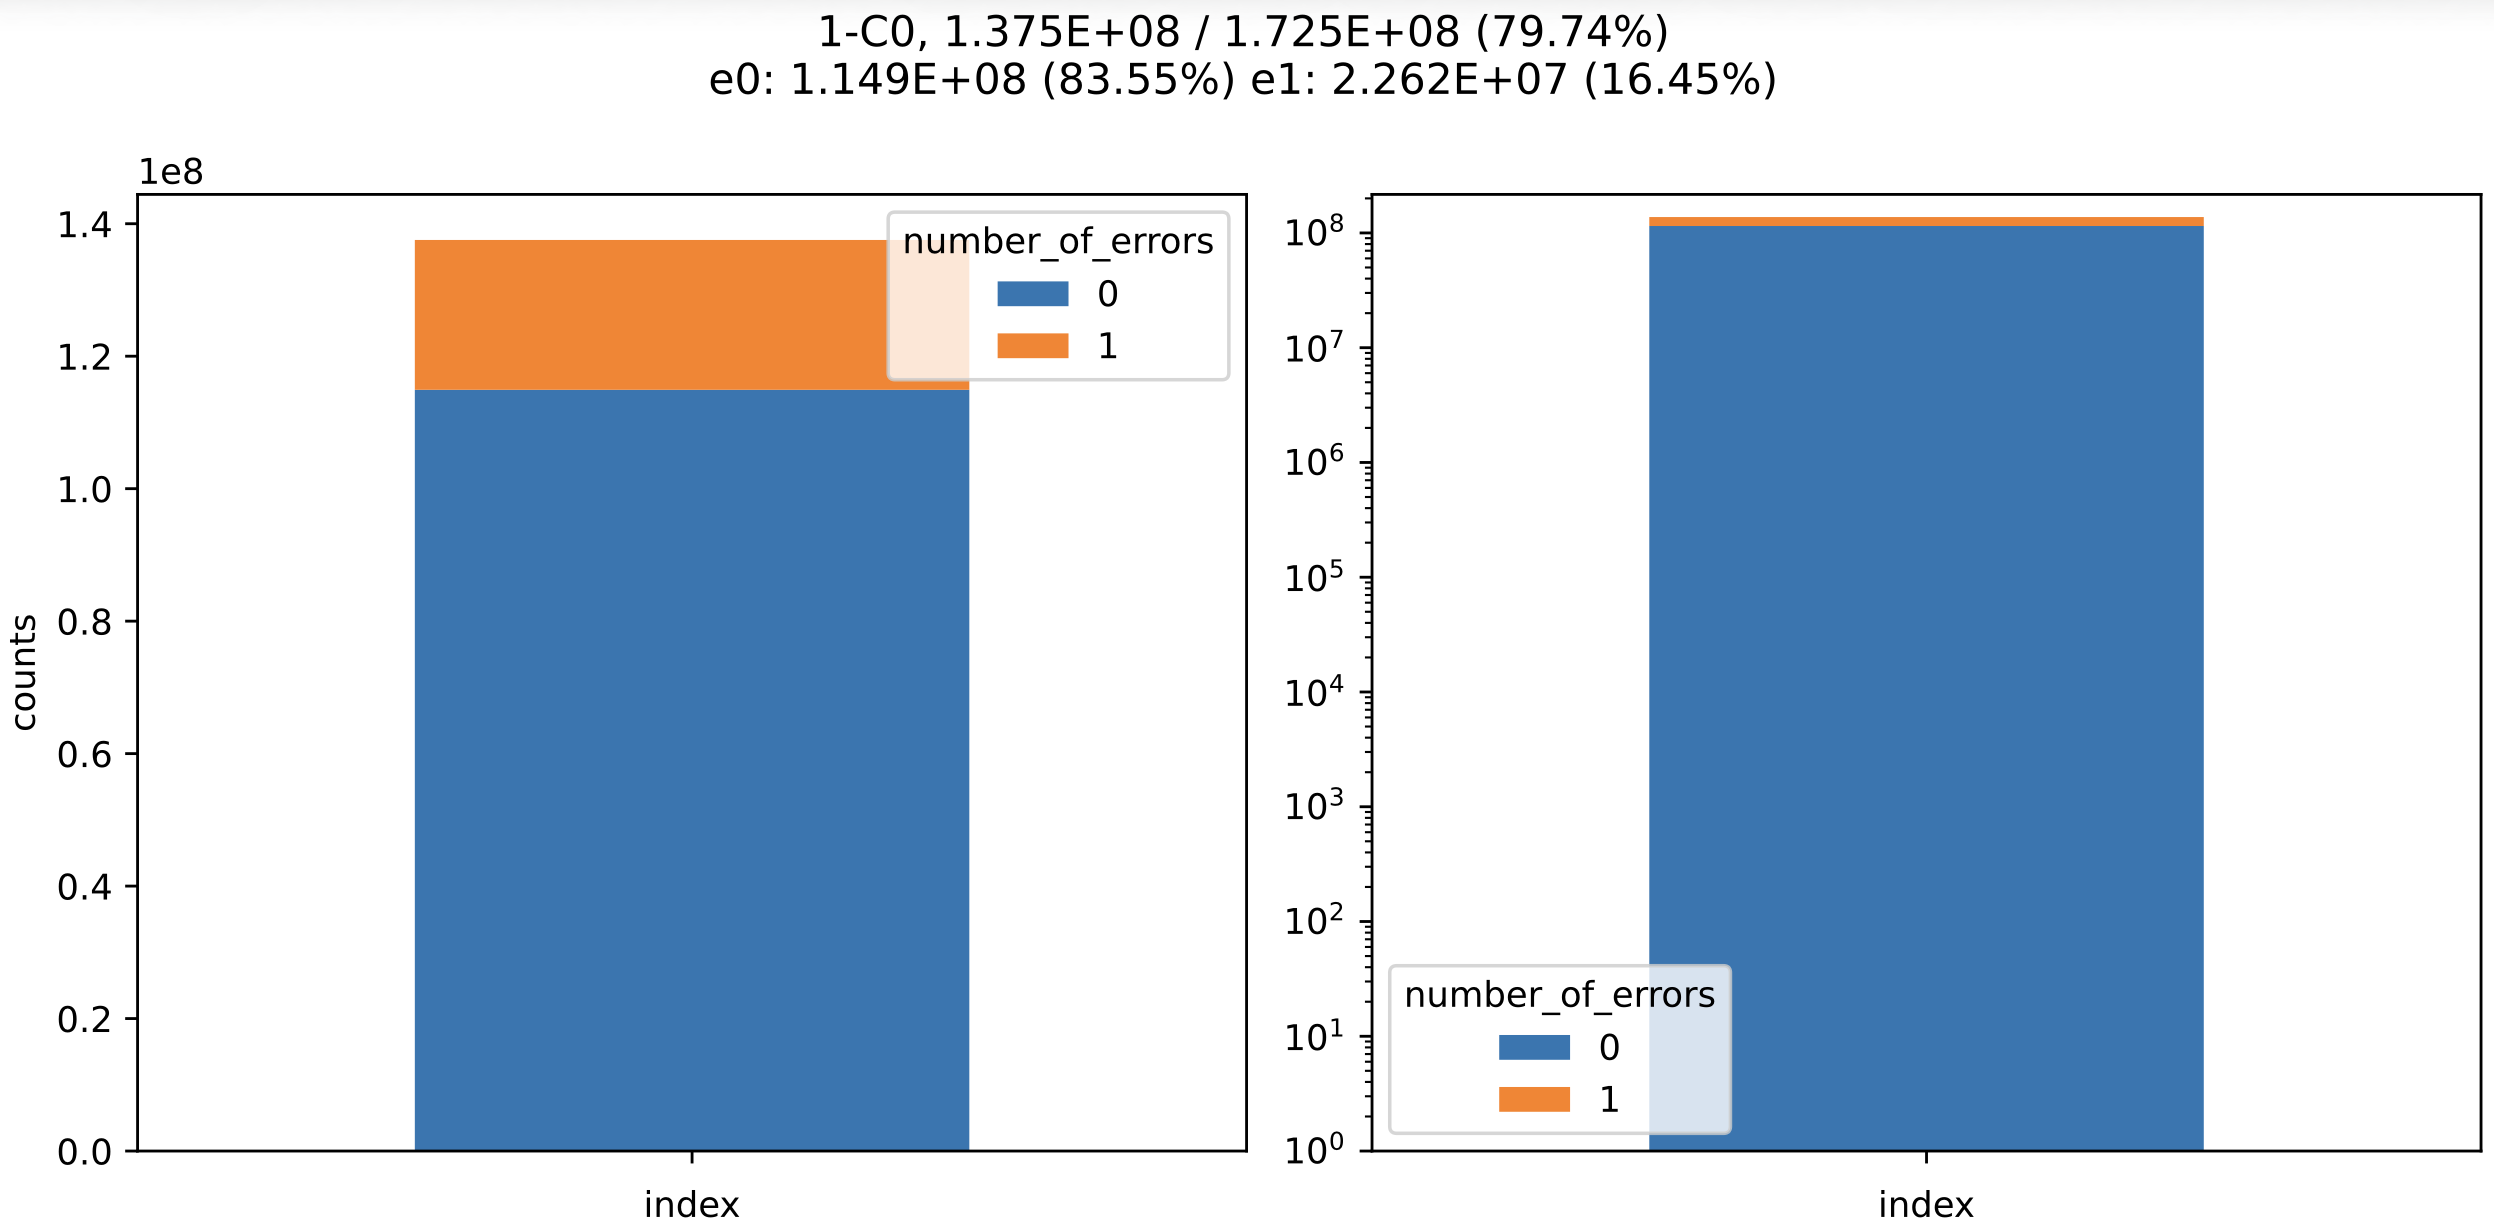
\includegraphics[width=\textwidth]{figures/image6.png}
\caption{Interactive dashboard interface. The dashboard provides interactive visualization of count data with filtering capabilities (not shown). The top panel shows experimental metadata (not shown), while the main panel displays count distributions and allows exploration of specific compounds.}
\label{fig:figure6}
\end{figure}
Using the dashboard:

\begin{itemize}
  \item Select different count files to visualize different selection conditions
  \item Visualize aggregated counts across codon dimensions:
  \item Apply filters to focus on specific count ranges
\end{itemize}
Note: The dashboard displays raw counts from the demultiplexing step. For statistical comparisons and hit identification, use the enrichment analysis results from Phase 5. The dashboard command accepts counts provided as a .txt file. Users can therefore perform their own custom normalization and simply point the dashboard to the resulting normalized counts.txt file for visualization by using --counts\_path and --selection\_name with the dashboard command.

CRITICAL: The default folder hierarchy as produced by delt-hit process needs to be used or if a custom counts.txt is provided the user needs to pass the selection name with as specified in the selection sheet as well.


\subsubsection{Phase 4: Selection-centric enumeration and analysis • TIMING 10 min - 2 h}
This phase generates chemical structures and calculates molecular properties for the top enriched compounds identified in a given selection. Library enumeration requires advanced knowledge of the SMARTS/SMIRKS language. While we provide common reaction patterns observed in DNA encoded libraries, library specific tweaks are often necessary.


\paragraph{Step 9 \textbar{} Enumerate top compounds from a selection}

Generate chemical structures for the top enriched compounds identified in a given selection. First visualize the reaction graph to verify the library architecture, then enumerate the top hits:


\begin{lstlisting}
delt-hit visualize enumerate --config_path=$CONFIG_PATH

delt-hit library enumerate \
  --config_path=$CONFIG_PATH \
  --counts_path=/path/to/selections/SELECTION/counts.txt \
  --top_n=1000 \
  --library_name=SELECTION_top_hits
\end{lstlisting}
Those commands:

\begin{itemize}
  \item Visualize the reaction graph of the library architecture for inspection
  \item Enumerate the top \texttt{top\_n} compounds by count for the specified selection
  \item Validates chemical structures
  \item Saves the compound catalog for the selected hits
\end{itemize}
Expected outputs:

\begin{itemize}
  \item library/SELECTION\_top\_hits/library.parquet: Compound catalog for the top hits with SMILES and barcode mappings
  \item reaction\_graph.png: Visual representation of synthetic schema
  \item additional\_reactions\_graph.png: Visualizes the additional reactions from the reaction\_graph sheet
  \item building\_block\_reactions\_graph.png: Visualizes the reactions derived from the building block sheets B0, B1, etc.
\end{itemize}

\begin{figure}[htbp]
\centering
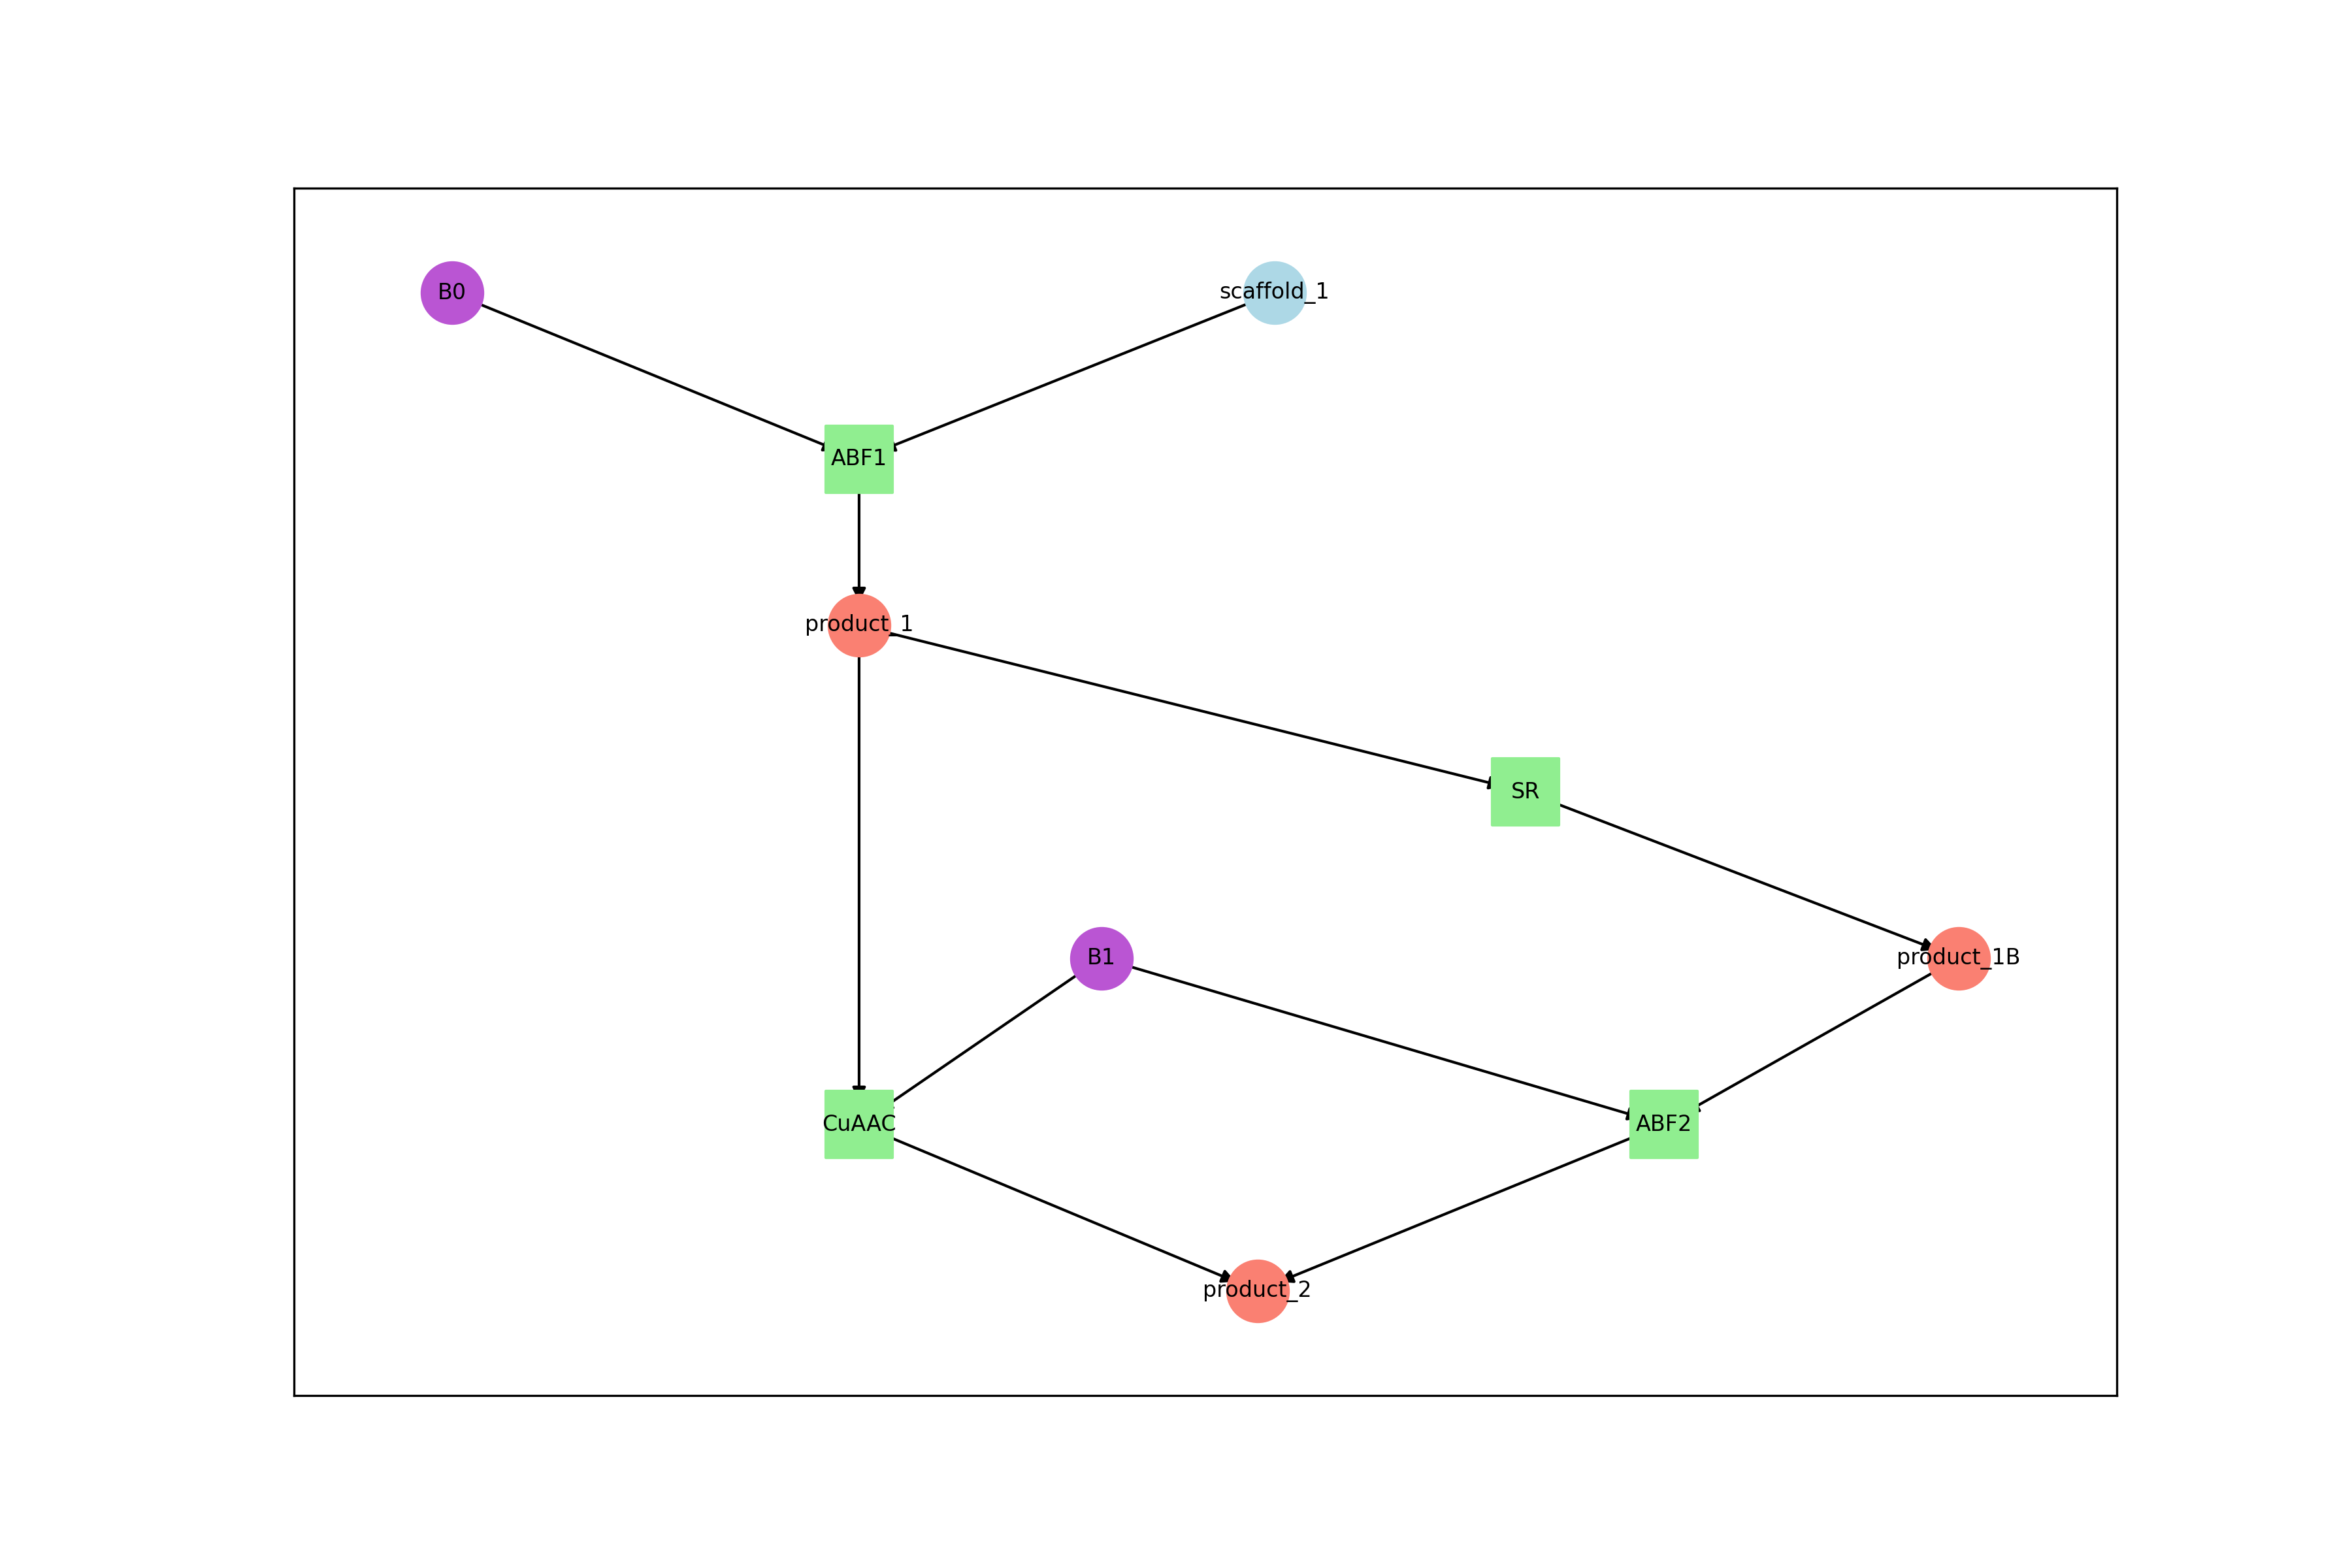
\includegraphics[width=\textwidth]{figures/image2.png}
\caption{Complete reaction graph for a DEL with two building blocks (violet), reactions (green), products (red) and starting compounds (blue).}
\label{fig:figure2}
\end{figure}
Performance: Enumeration speed is approximately 1’000-10’000 compounds/second depending on reaction complexity. For a 1 million compound library, expect 2-10 minutes of processing time depending on the machine.

TROUBLESHOOTING:

\begin{itemize}
  \item Check that all reaction SMIRKS are valid and specific enough to produce a single product
  \item Ensure reactant and product names match between building blocks and compounds sheets
  \item Re-run enumeration in debugging mode to visualize the reaction graphs that fail: delt-hit library enumerate --config\_path=/path/to/config.yaml --debug=invalid
\end{itemize}

\paragraph{Step 10 \textbar{} Visualize and calculate molecular properties of top hits}

Visualize the enumerated top hits and compute comprehensive molecular descriptors for drug-likeness assessment and chemical space characterization of the selected compounds:


\begin{lstlisting}
delt-hit visualize library --config_path=$CONFIG_PATH --library_name=SELECTION_top_hits
delt-hit library properties --config_path=$CONFIG_PATH --library_name=SELECTION_top_hits
\end{lstlisting}
Computed properties include:

\begin{itemize}
  \item Lipinski descriptors: Molecular weight (MW), partition coefficient (LogP), hydrogen bond donors (HBD), hydrogen bond acceptors (HBA)
  \item Topological indices: Topological polar surface area (TPSA), rotatable bonds
  \item Structural complexity metrics: Number of aromatic rings, heavy atom count, formal charge
  \item Drug-likeness scores: Quantitative estimate of drug-likeness (QED), fraction of sp³ carbons
\end{itemize}
Expected outputs:

\begin{itemize}
  \item properties/properties.parquet: Library catalog augmented with molecular descriptors
  \item properties/prop\_*.png: Distribution plots for each calculated property
\end{itemize}

\begin{figure}[htbp]
\centering
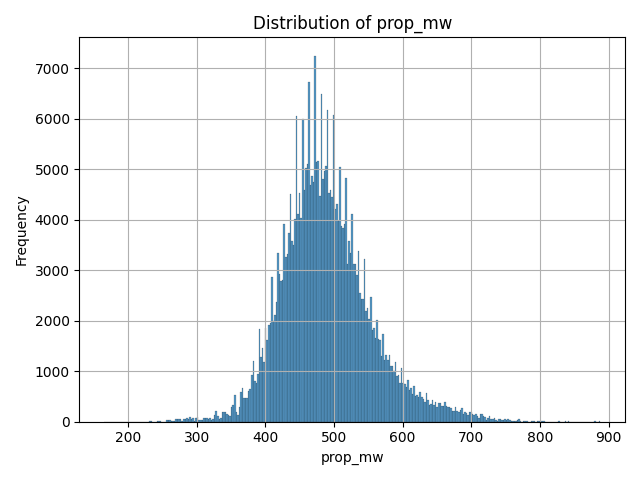
\includegraphics[width=\textwidth]{figures/image3.png}
\caption{Exemplary plot for the molecular weight distribution of library members.}
\label{fig:figure3}
\end{figure}
Performance note: Property calculation processes approximately 600-1000 compounds/second. For a 1 million compound library, expect 15-30 minutes processing time.


\subsubsection{Phase 5: Statistical analysis and hit identification • TIMING 10-30 min}
This phase identifies enriched library members by comparing selection conditions using established statistical methods.


\paragraph{Step 12 \textbar{} Define statistical comparisons}

From the information in the selections sheet, create a new dedicated configuration yaml file to specify which selections to compare.

A new configuration file is used to support comparisons across different selection runs, i.e. runs that might come from multiple individual sequencing files.


\begin{lstlisting}
# new analysis.yaml
experiments:
- name: protein_vs_no_protein
  save_dir: /Volumes/experiment-GB/analysis
  selections:
    - name: AG24_4
      counts_path: /Volumes/experiment-GB/selections/AG24_4/counts.txt
      group: no_protein
    - name: AG24_5
      counts_path: /Volumes/experiment-GB/selections/AG24_5/counts.txt
      group: no_protein
    - name: AG24_6
      counts_path: /Volumes/experiment-GB/selections/AG24_6/counts.txt
      group: no_protein
    - name: AG24_13
      counts_path: /Volumes/experiment-GB/selections/AG24_13/counts.txt
      group: protein
    - name: AG24_14
      counts_path: /Volumes/experiment-GB/selections/AG24_14/counts.txt
      group: protein
    - name: AG24_15
      counts_path: /Volumes/experiment-GB/selections/AG24_15/counts.txt
      group: protein
\end{lstlisting}

\paragraph{Step 13 \textbar{} Perform enrichment analysis with statistical methods}

DELT-Hit supports two statistical approaches for identifying enriched compounds. Both methods generate an Rscript that can be executed and/or further modified by the user.

Method 1: Simple counts method (suitable for single replicates)


\begin{lstlisting}
# Generate R script for counts-based analysis
delt-hit analyse enrichment --config_path=/path/to/analysis-config.yaml --name=protein_vs_no_protein --method=counts

# Execute the generated R script
Rscript --vanilla /path/to/experiment/analyses/analysis-1/counts/enrichment_counts.R
\end{lstlisting}
The counts method:

\begin{itemize}
  \item Averages counts across replicates within each group
  \item Computes simple differences between groups
  \item Does not provide statistical significance testing
  \item Suitable for exploratory analysis or when replicates are not available
\end{itemize}
Method 2: edgeR method (recommended when replicates are available)


\begin{lstlisting}
# Generate R script for edgeR statistical analysis
delt-hit analyse enrichment --config_path=/path/to/analysis-config.yaml --name=protein_vs_no_protein --method=edgeR


# Execute the generated R script
Rscript --vanilla /path/to/experiment/analyses/analysis-1/edgeR/enrichment_edgeR.R
\end{lstlisting}
The edgeR method:

\begin{itemize}
  \item Implements sophisticated RNA-seq-derived statistical models
  \item Uses empirical Bayes shrinkage for improved power
  \item Calculates false discovery rate (FDR) corrected p-values
  \item Requires replicates (minimum 2 per group)
  \item Provides normalized count tables
\end{itemize}
For both methods, the tool produces the Rscripts that implement the corresponding analysis. This enables users to easily further customize their analysis pipelines.

Expected outputs (both methods):

\begin{itemize}
  \item stats.csv: Complete statistics for all library members with columns:
  \item code\_1, code\_2, etc.: Building block indices
  \item LogFC: Log2 fold-change (edgeR) or difference in mean counts (counts method)
  \item PValue: Raw p-value (edgeR only)
  \item FDR: False discovery rate corrected p-value (edgeR only)
  \item enrichment\_hits.csv: Top enriched compounds (FDR \textless{} 0.05 for edgeR)
  \item correlation\_*.png: Replicate correlation plots for quality control
  \item Normalized count files for each selection or group
\end{itemize}
Interpreting results:

\begin{itemize}
  \item LogFC \textgreater{} 0: Compound enriched in protein selections vs controls
  \item LogFC \textless{} 0: Compound depleted in protein selections vs controls
  \item FDR \textless{} 0.05: Statistically significant enrichment (edgeR only)
  \item High replicate correlation (R² \textgreater{} 0.7) indicates good experimental consistency
\end{itemize}
CRITICAL STEP: Always examine replicate correlation plots to verify data quality before interpreting hit lists. Poor correlation may indicate technical problems or batch effects.

TROUBLESHOOTING: If no hits are identified:

\begin{itemize}
  \item Check that experimental groups are correctly assigned
  \item Verify sufficient sequencing depth (\textgreater{}100 reads per compound for reliable statistics)
  \item Consider adjusting FDR threshold for exploratory analysis
  \item Examine correlation plots for replicate consistency issues
\end{itemize}
\begin{itemize}
  \item Figure 7 \textbar{} Replicate–replicate correlation of library member counts for quality control. Diagonal panels show density estimates of counts within each selection. Lower triangular panels report pairwise correlation coefficients between replicates. Upper triangular panels display scatter plots comparing counts from one replicate against another.
\end{itemize}

\begin{table}[htbp]
\centering
\caption{Hit identification by edgeR. Shown compounds are for FDR\textless{}0.05 and sorted by logFC to identify the top hits.}
\label{tab:table12}
\begin{tabular}{lllllll}
\toprule
code\_1 & code\_2 & logFC & logCPM & LR & PValue & FDR \\
\midrule
94 & 472 & 9.76658103 & 4.65399379 & 140.973181 & 1.63E-32 & 2.99E-29 \\
94 & 337 & 9.52452422 & 4.41931582 & 128.115071 & 1.06E-29 & 9.38E-27 \\
250 & 250 & 9.50138143 & 4.39920396 & 136.048263 & 1.95E-31 & 2.62E-28 \\
250 & 523 & 9.46551754 & 4.36448577 & 134.035088 & 5.37E-31 & 6.34E-28 \\
94 & 364 & 9.29500646 & 4.19806216 & 117.172728 & 2.63E-27 & 1.35E-24 \\
250 & 208 & 9.2845154 & 5.99659857 & 173.194896 & 1.48E-39 & 2.05E-35 \\
250 & 337 & 9.06687397 & 3.98375428 & 115.539372 & 6.00E-27 & 2.80E-24 \\
94 & 341 & 8.99590166 & 3.91723403 & 113.847311 & 1.41E-26 & 6.00E-24 \\
250 & 414 & 8.99240694 & 3.90981012 & 105.694583 & 8.60E-25 & 2.69E-22 \\
250 & 96 & 8.92430743 & 8.02773969 & 203.793994 & 3.10E-46 & 2.36E-41Phase 2: Chemical library enumeration and analysis • TIMING 10 min - 2 h This phase generates all possible chemical structures from your building block combinations and calculates molecular properties for downstream analysis. Library enumeration requires advanced knowledge of the SMARTS/SMIRKS language. While we provide common reaction patterns observed in DNA encoded libraries, library specific tweaks are often necessary. Step 4 \textbar{} Enumerate library compounds from building blocks Generate all possible chemical structures by combining building blocks according to the defined reaction schemes: delt-hit library enumerate --config\_path=/path/to/config.yaml --graph\_only=True  \# produce reaction graph only for inspection delt-hit library enumerate --config\_path=/path/to/config.yaml Those commands: Construct a reaction graph from your building blocks and reactions Enumerates all valid compound combinations Validates chemical structures Saves the complete library catalog  Expected outputs: library.parquet: Complete compound catalog with SMILES and barcode mappings reaction\_graph.png: Visual representation of synthetic schema additional\_reactions\_graph.png: Visualizes the additional reactions from the reaction\_graph sheet building\_block\_reactions\_graph.png: Visualizes the reactions derived from the building block sheets B0, B1, etc.  Figure 2 \textbar{} Complete reaction graph for a DEL with two building blocks (violet), reactions (green), products (red) and starting compounds (blue).   Performance: Enumeration speed is approximately 1’000-10’000 compounds/second depending on reaction complexity. For a 1 million compound library, expect 2-10 minutes of processing time depending on the machine. TROUBLESHOOTING: Check that all reaction SMIRKS are valid and specific enough to produce a single product Ensure reactant and product names match between building blocks and compounds sheets Re-run enumeration in debugging mode to visualize the reaction graphs that fail: delt-hit library enumerate --config\_path=/path/to/config.yaml --debug=invalid  Step 5 \textbar{} Calculate molecular properties and descriptors Compute comprehensive molecular descriptors for drug-likeness assessment and chemical space characterization: delt-hit library properties --config\_path=/path/to/config.yaml Computed properties include: Lipinski descriptors: Molecular weight (MW), partition coefficient (LogP), hydrogen bond donors (HBD), hydrogen bond acceptors (HBA) Topological indices: Topological polar surface area (TPSA), rotatable bonds Structural complexity metrics: Number of aromatic rings, heavy atom count, formal charge Drug-likeness scores: Quantitative estimate of drug-likeness (QED), fraction of sp³ carbons Expected outputs: properties/properties.parquet: Library catalog augmented with molecular descriptors properties/prop\_*.png: Distribution plots for each calculated property  Figure 3 \textbar{} Exemplary plot for the molecular weight distribution of library members.  Performance note: Property calculation processes approximately 600-1000 compounds/second. For a 1 million compound library, expect 15-30 minutes processing time. Step 6 \textbar{} Generate molecular representations for machine learning Create standardized chemical representations compatible with machine learning frameworks: \# Morgan fingerprints for similarity analysis \# \textasciitilde\{\}600-1000 compounds/s delt-hit library represent --method=morgan --config\_path=/path/to/config.yaml  \# BERT embeddings for deep learning applications \# \textasciitilde\{\}600-1000 compounds/s delt-hit library represent --method=bert --config\_path=/path/to/config.yaml Available representation methods: morgan: Morgan circular fingerprints (2048-bit vectors) for similarity searching and clustering bert: Transformer-based molecular embeddings (768-dimensional vectors) for deep learning Expected outputs: representations/morgan.npz: Sparse matrix of Morgan fingerprints representations/bert.npz: Dense matrix of BERT embeddings Note: These representations are compatible with scikit-learn, PyTorch, and TensorFlow for downstream machine learning applications. \\
\bottomrule
\end{tabular}
\end{table}


\subsubsection{Phase 6: Full library enumeration and machine learning representations • TIMING 1 h - 8 h}
This phase performs full library enumeration and generates molecular representations for downstream machine learning applications. These steps are optional and only required for ML workflows.

\paragraph{Step 12 \textbar{} Enumerate the full library}

Enumerate all library members for downstream machine learning tasks:

\begin{lstlisting}
delt-hit library enumerate --config_path=$CONFIG_PATH
\end{lstlisting}

\paragraph{Step 13 \textbar{} Calculate molecular properties for the full library}

Calculate molecular properties for all library members:

\begin{lstlisting}
delt-hit library properties --config_path=$CONFIG_PATH
\end{lstlisting}

\paragraph{Step 14 \textbar{} Generate molecular representations for machine learning}

Create standardized chemical representations compatible with machine learning frameworks:


\begin{lstlisting}
# Morgan fingerprints for similarity analysis
# ~600-1000 compounds/s
delt-hit library represent --method=morgan --config_path=/path/to/config.yaml

# BERT embeddings for deep learning applications
# ~600-1000 compounds/s
delt-hit library represent --method=bert --config_path=/path/to/config.yaml
\end{lstlisting}
Available representation methods:

\begin{itemize}
  \item morgan: Morgan circular fingerprints (2048-bit vectors) for similarity searching and clustering
  \item bert: Transformer-based molecular embeddings (768-dimensional vectors) for deep learning
\end{itemize}
Expected outputs:

\begin{itemize}
  \item representations/morgan.npz: Sparse matrix of Morgan fingerprints
  \item representations/bert.npz: Dense matrix of BERT embeddings
\end{itemize}
Note: These representations are compatible with scikit-learn, PyTorch, and TensorFlow for downstream machine learning applications.


\subsection{Troubleshooting}
This section provides solutions to common issues encountered during DELT-Hit analysis.


\begin{table}[htbp]
\centering
\caption{Common issues and solutions}
\label{tab:table13}
\begin{tabular}{p{2.4cm}p{3.2cm}p{4.0cm}p{5.0cm}}
\toprule
Step & Problem & Possible Cause & Solution \\
\midrule
Experimental setup & command not found: conda & Conda is not installed or not initialized in the shell environment. & Install Conda as described in the Experimental setup section and make sure Conda is initialized in your terminal session. On Mac this typically is done by \textasciitilde\{\}/miniconda3/bin/activate and Windows with \textasciitilde\{\}/miniconda3/etc/profile.d/conda.sh \\
9 & Command fails with unrecognized arguments & Trailing spaces after \textbackslash\{\} when using multiline commands; Mistyped the command & Ensure that multiline commands do not have trailing spaces and ensure that the delt-hit commands are correctly typed. You can find more information for each command by typing delt-hit \textless{}cmd\textgreater{} --help \\
9 & Demultiplexing fails No such file or directory: '.../input.fastq.gz' & Trailing whitespaces in the file name in as defined in the excel sheet experiment & Remove any whitespaces and spaces in the file name and regenerate the config file with the delt-hit init command \\
13 & Low demultiplexing efficiency (\textless{}50\%) & Incorrect barcode sequences, inverted barcode sequences & Increase max\_error\_rate parameters; validate barcode sequences against sequencing data; check for adapter contamination \\
13 & qc/report.txt does not open & Text Editor does not support the encoding. & To show the content use the terminal and the cat command: cat qc/report.txt \\
Experimental setup / 18 & R script failures & Missing R packages, R not available in environment & Reinstall R into conda environment; reinstall R packages using BiocManager; verify R installation with which R; check R version (4.1+ required) \\
18 & Empty hit lists & Stringent statistical thresholds & Adjust FDR cutoffs (try 0.1 or 0.2 for exploratory analysis); check replicate consistency \\
15 & Chemical structure errors & Invalid SMILES, incorrect reaction SMIRKS & Validate building block structures using RDKit; check reaction definitions; test reactions with a small building block subset; run enumeration in debug mode \\
Experimental setup & "Command not found" errors & Conda environment not activated & Run conda activate delt-hit before executing DELT-Hit commands \\
11 & Permission denied for shell scripts & Executable permission not set & Run chmod u+x \textless{}script\_name.sh\textgreater{} before executing shell scripts \\
18 & Poor replicate correlation & Batch effects, technical variability & Review selection protocol for consistency; check for contamination \\
\bottomrule
\end{tabular}
\end{table}


\subsubsection{Performance optimization guidelines}
Memory requirements by library size:

\begin{itemize}
  \item Small libraries (\textless{}1M compounds): 16 GB RAM sufficient
  \item Medium libraries (1-50M compounds): 32GB RAM recommended
  \item Large libraries (\textgreater{}50M compounds): 32GB RAM required
\end{itemize}
Processing speed optimization:

\begin{itemize}
  \item Use SSD storage for faster I/O operations
  \item Increase num\_cores parameter for parallel processing
  \item Use compressed FASTQ files (.gz) to reduce disk space
\end{itemize}

\subsubsection{Quality control thresholds}
Demultiplexing quality indicators:

\begin{itemize}
  \item Excellent: \textgreater{}90\% initial read retention
  \item Good: 70-90\% initial retention
  \item Acceptable: 50-70\% initial retention
  \item Poor: \textless{}50\% retention (requires troubleshooting)
\end{itemize}
Statistical analysis quality indicators:

\begin{itemize}
  \item Replicate correlation: R² \textgreater{}0.7 for biological replicates (R² \textgreater{}0.9 for technical replicates)
  \item Positive / negative controls: That positive and negative controls give expected outputs
\end{itemize}

\subsection{Timing}
Protocol execution times depend on dataset characteristics and computational resources. This table provides estimates for different dataset scales using the recommended hardware configuration (32 GB RAM, 16 CPU cores).


\begin{table}[htbp]
\centering
\caption{Timing estimates for different dataset sizes}
\label{tab:table14}
\begin{tabular}{llll}
\toprule
Analysis Phase & Small Dataset¹ & Medium Dataset² & Large Dataset³ \\
\midrule
Software installation (one-time) & 15-30 min & 15-30 min & 15-30 min \\
Project initialization & 15-30 min & 15-60 min & 60-120 min \\
Library enumeration & 2-5 min & 15-45 min & 1-2 h \\
Property calculation & 1-3 min & 10-30 min & 30 min-1 h \\
Molecular representation & 2-5 min & 15-45 min & 45 min-1.5 h \\
Sequence demultiplexing & 10-30 min & 1-2 h & 2-6 h \\
Statistical analysis & 2-5 min & 5-15 min & 15-45 min \\
Visualization and interpretation & 5-15 min & 10-30 min & 15-45 min \\
Total workflow time & 45 min-1.5 h & 2-4 h & 4-10 h \\
\bottomrule
\end{tabular}
\end{table}
¹Small dataset: \textless{}100K compounds
²Medium dataset: 100K-10M compounds
³Large dataset: \textgreater{}10M compounds

Notes:

\begin{itemize}
  \item Software installation is required only once before first use
  \item Times assume recommended hardware configuration (32 GB RAM, 16 CPU cores)
  \item Parallel processing (num\_cores parameter) significantly affects timing
\end{itemize}

\subsection{Anticipated results}

\subsubsection{Output file structure}
DELT-Hit generates a comprehensive, standardized output hierarchy:


\begin{lstlisting}
project_root/
|---- analysis.yaml                        # analysis specification
|---- campaign.fastq.gz                    # Raw sequencing reads 
|---- template.xlsx                        # Input excel sheet 
|
`---- experiments/                         # experiments (one folder per campaign)
    `---- template/                        # Example experiment instance
        |---- config.yaml                  # Experiment-level config
        |
        |---- demultiplex/                 # Cutadapt-based demultiplexing)
        |   |---- cutadapt_input_files/    # Files passed to Cutadapt (generated)
        |   |   |---- demultiplex.sh       # Generated shell script running Cutadapt steps
        |   |   `---- {0-S0,1-C0,2-B0,...}.fastq   # Cutadapt adapter lists
        |   `---- cutadapt_output_files/   # Cutadapt outputs per step
        |       |---- *.cutadapt.json      # Per-step JSON stats from Cutadapt
        |       |---- *.cutadapt.log       # Per-step logs (stdout/stderr capture)
        |       |---- input.fastq.gz       # Cutadapt input for the demultiplexing
        |       |---- out.fastq.gz         # Cutadapt output for the demultiplexing
        |       `---- reads_with_adapters.gz  # Reads retained with adapters
        |
        |---- library/                     # Library reconstruction & enumeration outputs
        |   |---- library.parquet          # Enumerated library table
        |   |---- reaction_graph.png       # Main reaction graph visualization
        |   |---- building_block_reactions_graph.png   # Graph focused on building blocks
        |   |---- additional_reactions_graph.png       # Extra/optional reactions graph
        |   |
        |   `---- properties/              # Calculated molecular descriptors for the library
        |       |---- properties.parquet   # Descriptor table aligned with library.parquet
        |       `---- prop_*.png           # Descriptor distributions (e.g.,mw/logP/TPSA/QED/...)
        |
        |---- representations/             # ML-ready representations derived from SMILES
        |   |---- morgan.npz               # Morgan fingerprints (sparse array)
        |   `---- bert.npz                 # Embeddings (e.g., SMILES BERT)
        |
        |---- selections/                  # Per-selection count tables (from demultiplexing)
        |   |---- AG24_4/                  # One selection / condition / replicate
        |   |   `---- counts.txt           # Count table for this selection
        |   |---- AG24_5/
        |   |   `---- counts.txt
        |   |---- AG24_6/
        |   |   `---- counts.txt
        |   |---- AG24_13/
        |   |   `---- counts.txt
        |   `---- ...                      # Many more selections
        |   # Note: AG24_*_counts.txt files at this level are flattened copies of the per-  
        |           folder counts
        |
        |---- qc/                          # Quality control outputs
        |   |---- report.txt               # Human-readable QC summary
        |   |---- hits_{0-S0,1-C0,2-B0,...}.parquet  # Per-step ?hit? tables
        |   `---- hits_{0-S0,1-C0,2-B0,...}.pdf      # Per-step QC report plots
        |
        `---- analysis/                    # Downstream statistical analyses
            `---- protein_vs_no_protein/   # One analysis definition (experiment name)
                |---- samples.csv          # metadata for statistical analysis
                |---- data.csv             # data for statistical analysis
                |
                |---- counts/              # Simple counts-based enrichment
                |   |---- enrichment_counts.R          # Script to compute enrichment
                |   |---- stats.csv                    # Full results table
                |   |---- hits.csv                     # Filtered top hits
                |   |---- protein.csv                  # Group-normalized counts
                |   |---- no_protein.csv               # Group-normalized counts
                |   `---- correlation_{protein,no_protein}.png  # Replicate correlation plots
                |
                `---- edgeR/               # edgeR-based differential enrichment
                    |---- enrichment_edgeR.R           # edgeR workflow script
                    |---- enrichment_stats.csv         # Full results with p-values/FDR
                    |---- enrichment_hits.csv          # Significant hits (e.g., FDR < 0.05)
                    |---- {AG24_4,AG24_5,AG24_6,...}.csv  # Normalized counts per selection
                    `---- correlation_{protein,no_protein}.png  # Replicate correlation plots
\end{lstlisting}

\subsubsection{Chemical library characterization}
Library enumeration generates comprehensive structural and chemical space information for all possible compounds in your DEL.

Library enumeration:

The reaction graph (Figure 2) visualizes the synthetic scheme, showing how building blocks combine through defined reactions to generate final products. This representation helps validate:

\begin{itemize}
  \item Correct reaction connectivity
  \item Building block incorporation at each step
  \item Expected product formation
\end{itemize}
Library size:

\begin{itemize}
  \item Library enumeration should produce as many compounds as expected for the provided library setup.
\end{itemize}
Molecular property distributions:

Property calculation provides comprehensive descriptor analysis for drug-likeness assessment. Figure 3 shows a typical molecular weight distribution with most compounds falling in the 300-600 Da range.


\subsubsection{Demultiplexing performance}
Successful demultiplexing indicates high-quality library and sequencing data.

Quality control visualizations (Figures 4 - 5) show:

\begin{itemize}
  \item Read retention through processing steps: Tracks the percentage of reads retained after each adapter trimming step
  \item Barcode coverage distributions: Displays how evenly reads are distributed across building blocks
  \item Error rate distributions: Shows the frequency of sequencing errors detected at each position
\end{itemize}
Performance interpretation:

\begin{itemize}
  \item Excellent/Good performance: Library is well constructed with high-quality sequencing
  \item Acceptable performance: Usable for analysis but may have reduced sensitivity
  \item Poor performance: Indicates technical issues requiring troubleshooting (see Troubleshooting section)
\end{itemize}
Common patterns:

\begin{itemize}
  \item High initial retention (\textgreater{}90\%): Correct adapter sequences, good sequencing quality
  \item Even barcode distribution: Well-balanced library without synthesis bias
  \item Low error rates (\textless{}2\%): High-quality sequencing suitable for stringent matching
\end{itemize}

\subsubsection{Statistical analysis outputs}
Hit identification provides ranked lists of enriched compounds with statistical significance assessment.

Expected enrichment patterns:

For a typical protein target screen against negative controls:

\begin{itemize}
  \item Dynamic range: 2-1000 fold enrichment over negative controls
  \item Replicate consistency: Pearson correlation R \textgreater{} 0.7 between biological replicates
  \item Statistical power: Reliable detection of \textgreater{}2-fold enrichment with \textgreater{}100 reads per compound
  \item Reproducible selection experiments
  \item Minimal batch effects
  \item Reliable statistical inference
\end{itemize}

\subsubsection{Integration capabilities and downstream applications}
DELT-Hit outputs integrate seamlessly with established cheminformatics and machine learning workflows.

Machine learning workflows:

The generated molecular representations enable:

\begin{itemize}
  \item Scikit-learn compatibility: Morgan fingerprints for classification, regression, and clustering
  \item Deep learning frameworks: BERT embeddings compatible with TensorFlow and PyTorch
  \item Chemical similarity analysis: Tanimoto similarity calculations using Morgan fingerprints
  \item Dimensionality reduction: PCA, t-SNE, or UMAP visualization of chemical space
\end{itemize}
Cheminformatics pipelines:

Integration with RDKit and other tools for:

\begin{itemize}
  \item Structure-activity relationship (SAR) analysis: Identification of structural motifs associated with activity
  \item Virtual screening: Use enriched compounds to search larger chemical databases
\end{itemize}
Statistical analysis:

Direct export to R for specialized modeling:

\begin{itemize}
  \item Dose-response modeling: Analyze enrichment across multiple selection stringencies
  \item Multi-target analysis: Compare enrichment patterns across different protein targets
\end{itemize}

\subsection{Data and code availability}

\subsubsection{Software access and documentation}
DELT-Hit software is freely available under MIT License:

\begin{itemize}
  \item Primary repository: https://github.com/DELTechnology/delt-hit
  \item Installation: pip install git+https://git@github.com/DELTechnology/delt-hit.git
  \item Documentation: Comprehensive user guides, API reference, and tutorials at the repository
  \item Issue tracking: Community support and bug reporting via GitHub Issues
\end{itemize}

\subsection{Author contributions}
A.M. conceived the project, designed the software architecture, and implemented core algorithms. A.L. created and maintained the configuration files and testing frameworks. G.H implemented core algorithms. A.G. performed selection experiments and helped with result interpretation. L.P. performed software validation and contributed to code fine-tuning. J.S. provided scientific oversight and experimental validation. All authors contributed to manuscript preparation and revision.


\subsection{Competing interests}
The authors declare no competing financial interests.


\subsection{Acknowledgments}
We thank the DEL research community for valuable feedback during software development and beta testing. We acknowledge the developers of Cutadapt, RDKit, edgeR, and other open-source tools that enable this framework. Special thanks to early adopters who provided critical feedback for improving usability and robustness.





\bibliographystyle{unsrt}
\bibliography{references}
\end{document}
